\documentclass[11pt, twocolumn]{article}
\usepackage{bnaic}
\usepackage[ruled,vlined]{algorithm2e}
\usepackage{graphicx}
\usepackage{caption}
\usepackage{subcaption}
\usepackage{adjustbox}
\usepackage{pdflscape}
\usepackage{float}
\usepackage{hyperref}
\usepackage{lipsum}
\usepackage{comment}
\usepackage{iftex}

\usepackage{fancyhdr}
\fancypagestyle{firstpage}
{
    \renewcommand{\headrulewidth}{0pt}
    \setlength{\headheight}{60pt} 
    \fancyhead[C]{
\includegraphics[width=14.5cm]{header/logo_rug_fse_ai.png}}
}


% \title{
\includegraphics[width=14.5cm]{header/logo_rug_fse_ai.png}\\\vspace{2cm}\textbf{\scshape{Bach Ex Machina}}}
\title{\vspace{1.5cm}\textbf{\scshape{Bach Ex Machina}}}
\author{
    Jorn van Wier\\
    \small j.h.a.van.wier@student.rug.nl
    
    \and 
    
    Ruurd Bijlsma\\
    \small r.bijlsma.3@student.rug.nl
    
    \and 
    
    Nischal Madiraju\\
    \small n.madiraju@student.rug.nl
    
    \and 
    
    Pranav Vallala\\
    \small p.g.vallala@student.rug.nl
}
\date{}

\pagestyle{plain}

\begin{document}

% \begin{figure*}[ht]
%     \centering
%     
\includegraphics[width=14.5cm]{header/logo_rug_fse_ai.png}
% \end{figure*}

\maketitle

\thispagestyle{firstpage}

\begin{abstract}
\noindent
The Art of the Fugue is Johann Sebastian Bach's incomplete musical work written in the last decade of his life. In this project, we are using multivariate LSTM and the MAESTRO dataset (V3.0.0) to generate 25 seconds of pseudo-Bach music that can serve as a part of Bach's unfinished fugue. 

In training our model we will use a loss function, but its very difficult to create a loss function that is able to determine whether music sounds 'good'. Therefore, for our final result, we will evaluate the sound manually to determine how well the model performed.

\end{abstract}
\section{Introduction}

\subsection{Problem}
% Jorn
In 1993 a time series prediction competition the Santa Fe Institute organized a time series prediction competition. One of the tasks for this competition was to complete a fugue by Johann Sebastian Bach, which was left unfinished as he died before completing his work. 
An analysis of the data for this task can be found in \cite{dirstt1993baroque}. In our work, we use an LSTM model to perform the same task. As deep learning techniques such as LSTM models benefit greatly from more input data, a richer dataset than the one for the Santa Fe competition would be very valuable.

\subsection{Dataset}
% Ruurd
To train our network we use the MAESTRO v3 dataset \cite{hawthorne2018enabling}. This dataset is composed of over 200 hours of piano performances captured with fine alignment (~3ms) between note labels and audio waveforms. The data consists of MIDI files recorded by a Yamaha Disklavier, a concert-quality acoustic grand piano. 
\par
The train/test split is provided by the authors of the dataset, this split is configured in a way such that the same composition does not appear in multiple subsets. The music in the dataset is mostly classical, including composed from the 17th to early 20th century.

\subsubsection{MIDI}
Our music generation method is based entirely around MIDI files. MIDI files provide a compact and real-world representation of instrumental audio, which makes them useful for our training purposes. A MIDI file can consist of one or more tracks. Each of these tracks contain messages, specifying events such as a piano key being pressed or released, or a piano foot paddle being pressed, along the metadata such as the velocity, pitch and precise timing. In the case of a piano, the velocity indicates how hard a key was pressed. 
\par
For our model, we transform the MIDI files to a simpler format. An entire MIDI file is converted to a 2D array with the pitch on one axis, and time on the other axis. This representation is visualized in \autoref{fig:represent}. In MIDI, the pitch is always an integer value between 0 and 128 (exclusive), therefore the size of the 2D array representation is always 128 x time units.
\begin{figure*}[h]
    \centering
    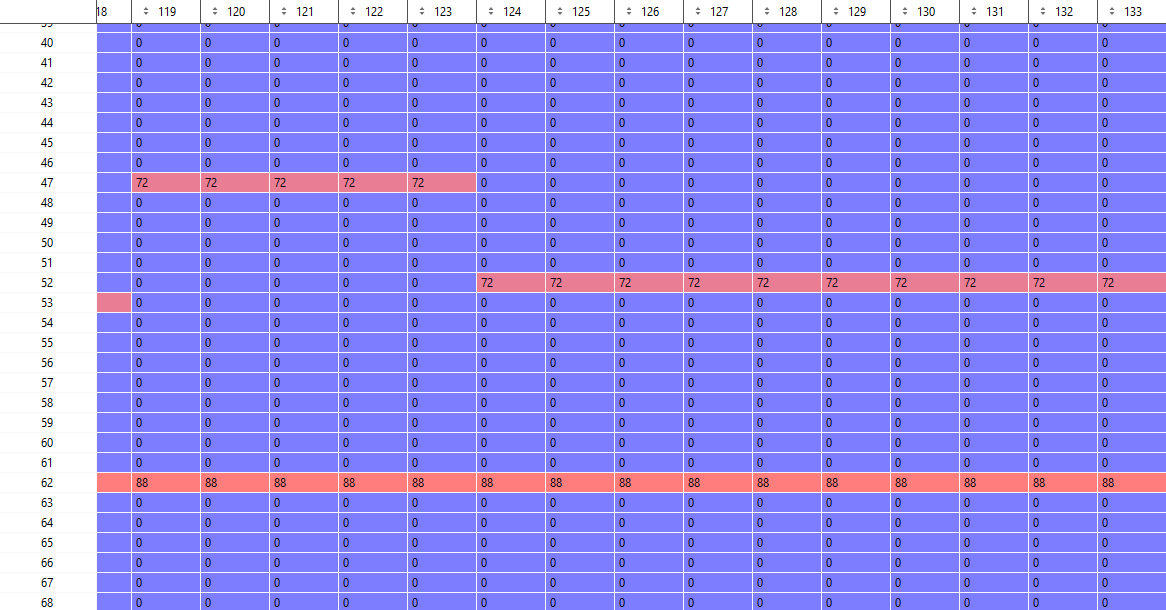
\includegraphics[width=\textwidth]{images/data.png}
    \caption{Example of a slice of the transformed MIDI file. The y-axis represents pitch, the x-axis represents time.}
    \label{fig:represent}
\end{figure*}
\par
The time units (ticks) used in MIDI are based on the tempo, which can change through each track, and a value called ticks per beat which is a constant value for each MIDI file. In our representation we simplify this by using our own ticks which always represent the same time unit (1/12th of a second) and assigning a velocity in the 2d array when at that timestamp a note was pressed at that level of pitch. For example, in \autoref{fig:represent}, a key was pressed for five ticks (from tick 119 to 123) with a pitch of 47, with a velocity of 72.
\par
By using this representation we merge all tracks present in the MIDI file into one format, therefore we support MIDI tracks with any number of tracks. 
Once we've transformed a MIDI file to this format we can feed it into a number of machine learning models, such as a hidden Markov model or an LSTM. Such models will then output in the same format, so we have also built a way to convert back from the simplified format to a MIDI file, which can be played by a synthesizer (or a computer).

\ifpdf
\else
\textbf{Generated using our hidden Markov model}

Original: Toto - Africa (piano version):

startaudio midi/sandstormpiano.wav endaudio

Generated audio using a hidden Markov model, based on Toto - Africa:

startaudio midi/standstormpredicted.wav endaudio

Original: Darude - Sandstorm (piano version):

startaudio midi/sandstormpiano.wav endaudio

Generated audio using a hidden Markov model, based on Darude - Sandstorm:

startaudio midi/standstormpredicted.wav endaudio
\fi
    
\subsection{Objectives}
% Pranav


\section{Methods}

\subsection{Baseline Model}
To help determine the success of our final LSTM model, we will compare it to a non-deep learning based model, namely a hidden Markov Model. We use a Gaussian hidden Markov model and train it on only the one input song, Bach's unfinished fugue. The velocities values of the simplified representation are not used in this model, as this lead to more chaotic results. By only feeding the model a 1 for a note pressed and a 0 for silence, we can threshold the output of the model and tune it to audibly produce better results.
% Hmm
\subsection{LSTM}

\lipsum[1-5]


\section{Results}
\section{Discussion}
 

\bibliographystyle{plain}
\bibliography{references}


\end{document}










